\documentclass[11pt,letterpaper]{article}

% Load some basic packages that are useful to have
% and that should be part of any LaTeX installation.
%
% be able to include figures
\usepackage{graphicx}
% get nice colors
\usepackage{xcolor}

% change default font to Palatino (looks nicer!)
\usepackage[latin1]{inputenc}
\usepackage{mathpazo}
\usepackage[T1]{fontenc}
% load some useful math symbols/fonts
\usepackage{latexsym,amsfonts,amsmath,amssymb}

% comfort package to easily set margins
\usepackage[top=1in, bottom=1in, left=1in, right=1in]{geometry}

% control some spacings
%
% spacing after a paragraph
\setlength{\parskip}{.15cm}
% indentation at the top of a new paragraph
\setlength{\parindent}{0.0cm}


\begin{document}

\begin{center}
\Large
Ay190 -- Worksheet 1\\
John Pharo\\
Date: \today\\
The Once and Future King: David Vartanyan
\end{center}

\section*{Problem 1}

The main body of the program runs in a for loop for a given number of timesteps (ntmax). In each iteration of the for loop, the code updates the artificial viscosity, the accelerations (and from this the velocities and half-step velocities), and the energy RHS. These are calculated using helper functions that take the current values and apply Equations IV.4.15 and IV.4.21 to find the new accelerations and energies. \\

Once these have been calculated, the loop updates the eps, velocity, and positions based on the current time step. Once this is done, it updates the list of neighboring particles, again through use of a helper function. Since this is a 1D problem, the neighbor search function just checks, for each particle, the number of particles within twice the smoothing length $h$ in either direction. \\

Having found the new neighbors, the loop then uses the information calculated thus far to recalculate the density, pressure, sound speed, and time step. The new timestep is essentially the ratio of the smoothing length to the sound speed, or 1.1 times the old step size, whichever is smaller. \\

Every fifth step, the loop updates the plot with the new dnesity distribution with radius. Below are some plot at various time steps (the time is printed in the upper-right corner), where you can watch the shock decay over time. After ~200 steps, the plot basically drops off to nothing.

\begin{figure}[bth]
\centering
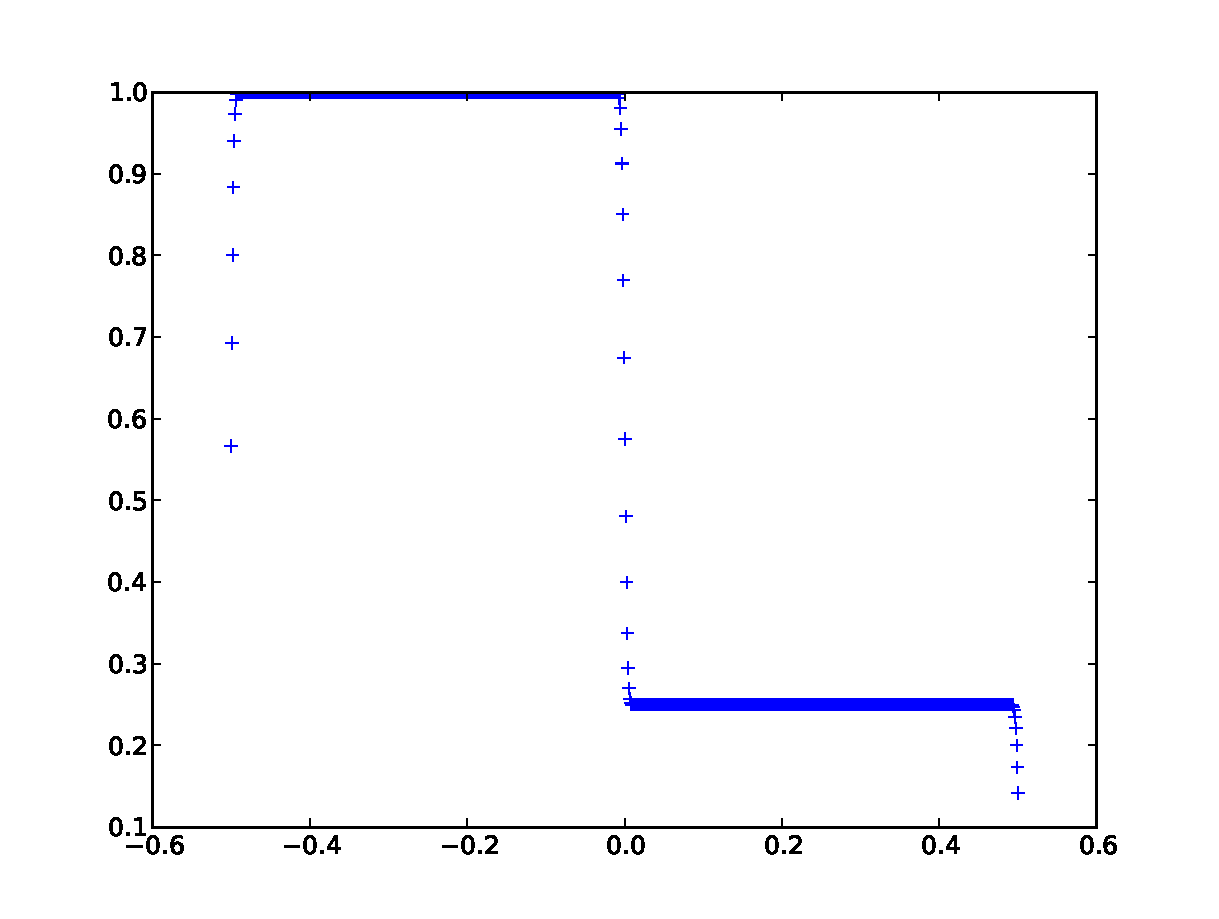
\includegraphics[width=0.5\textwidth]{Shock-1.pdf}
\label{fig:simpleplot}
\end{figure}

\begin{figure}[bth]
\centering
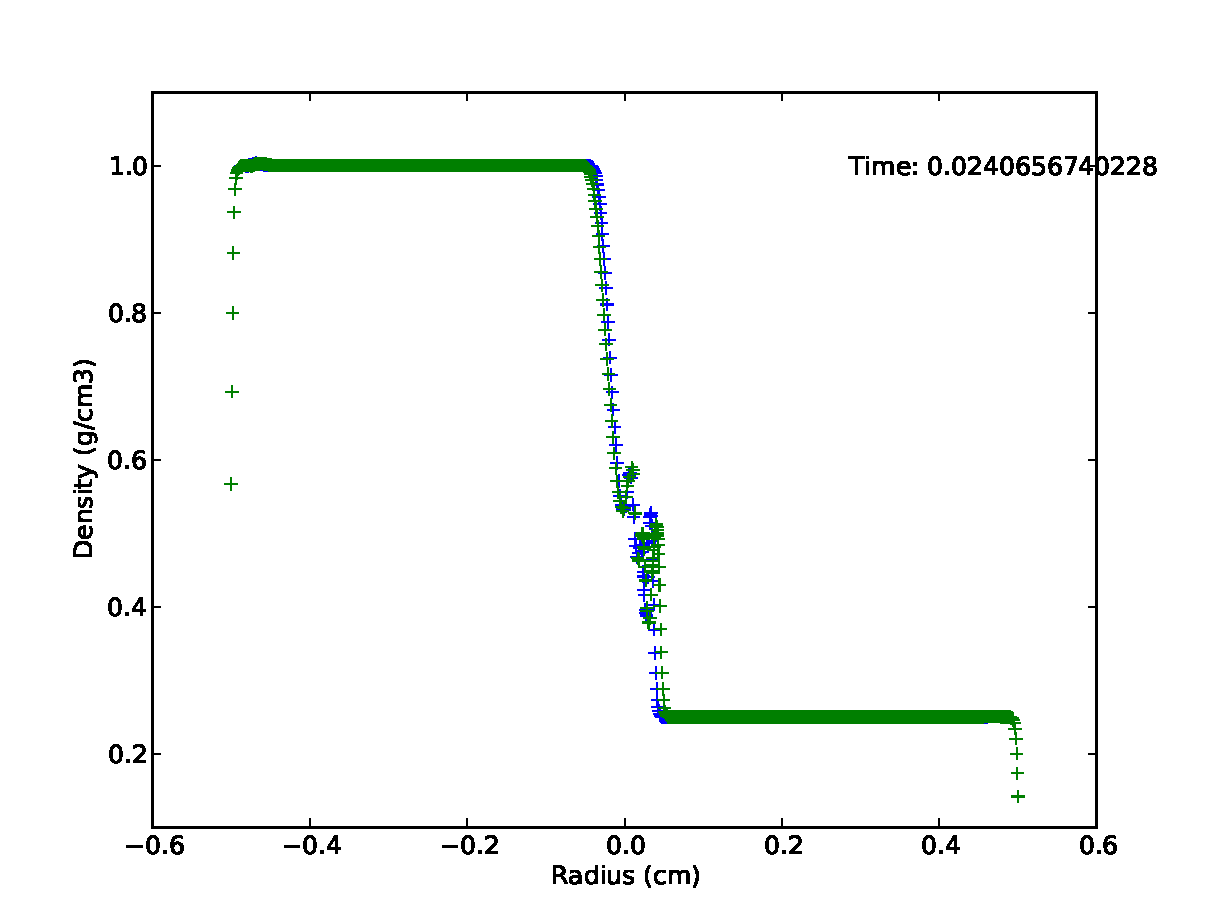
\includegraphics[width=0.5\textwidth]{Shock-25.pdf}
\label{fig:simpleplot}
\end{figure}

\begin{figure}[bth]
\centering
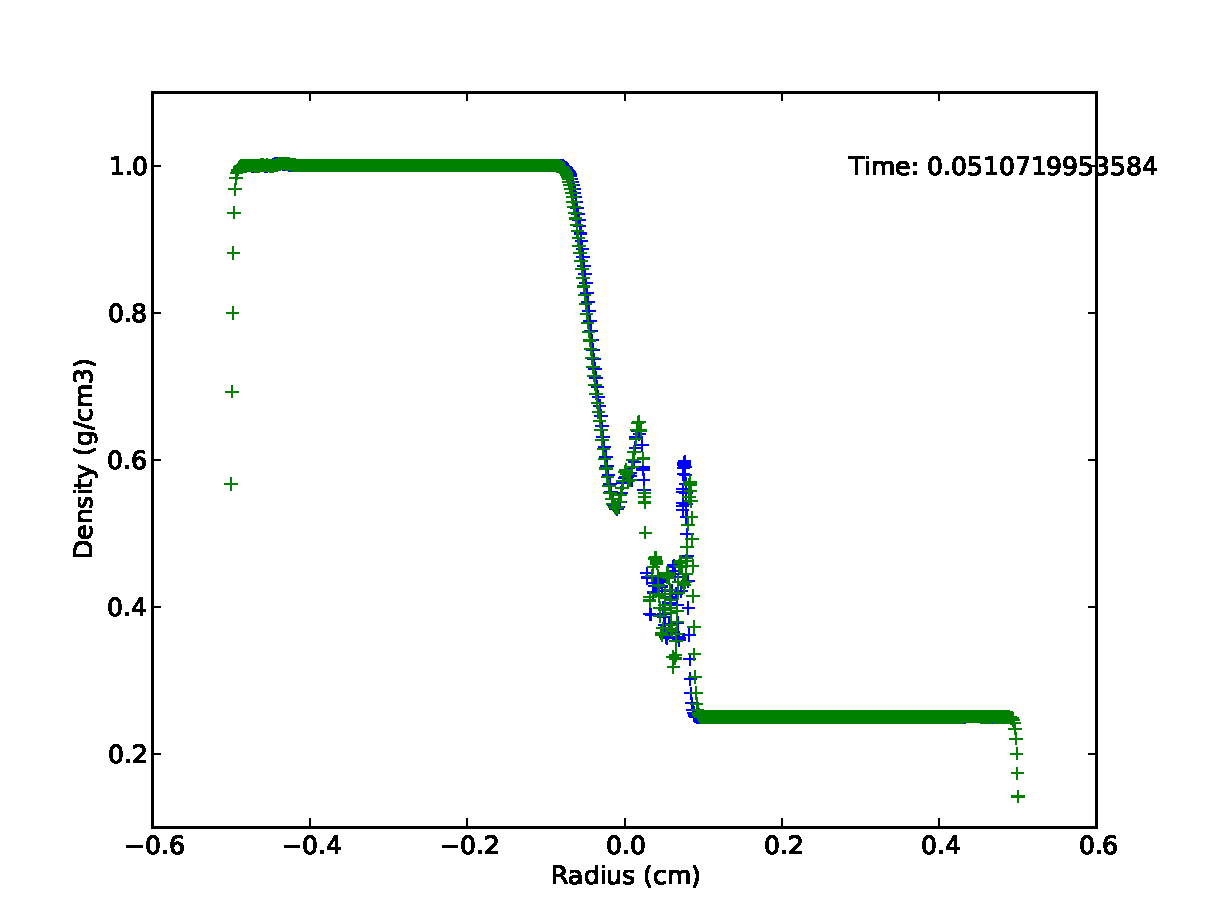
\includegraphics[width=0.5\textwidth]{Shock-50.pdf}
\label{fig:simpleplot}
\end{figure}

\begin{figure}[bth]
\centering
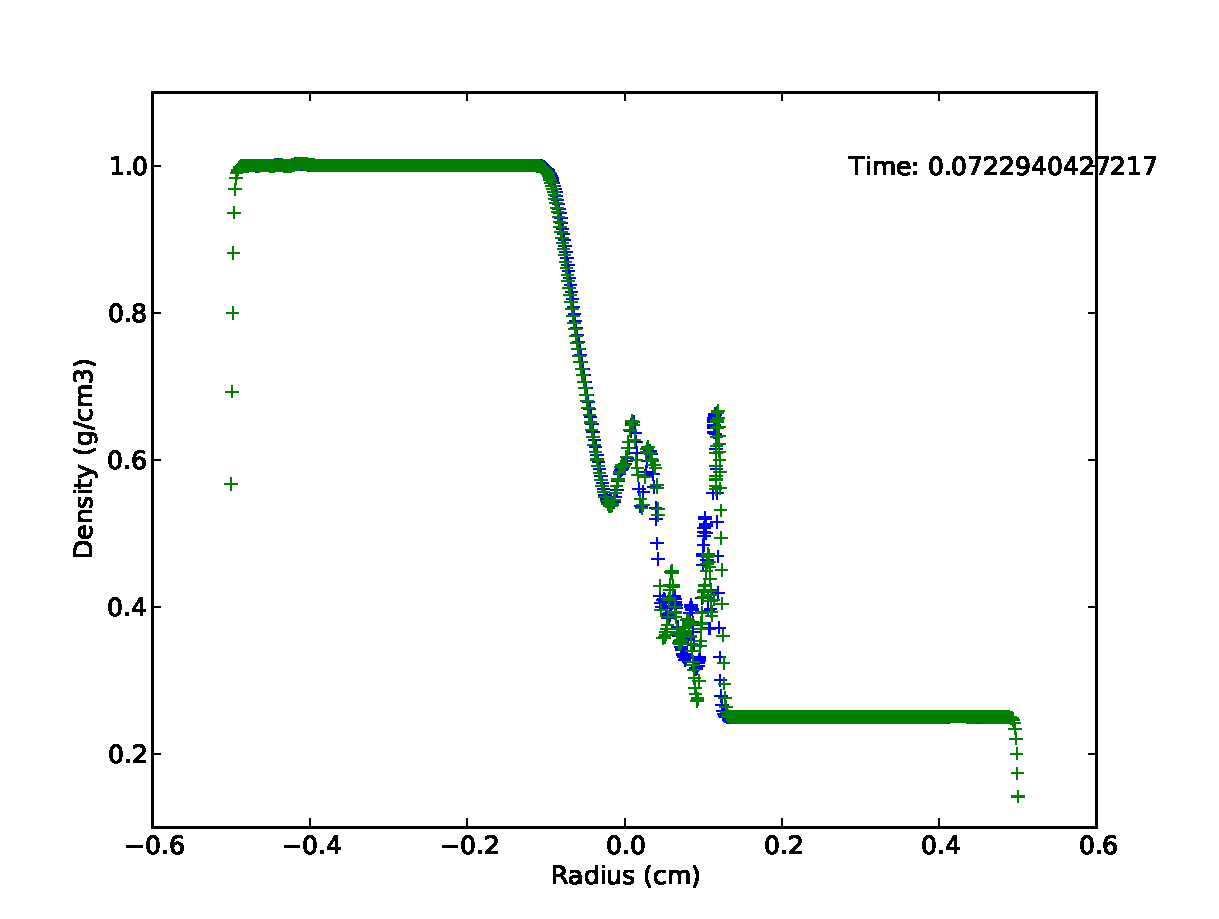
\includegraphics[width=0.5\textwidth]{Shock-75.pdf}
\label{fig:simpleplot}
\end{figure}

\begin{figure}[bth]
\centering
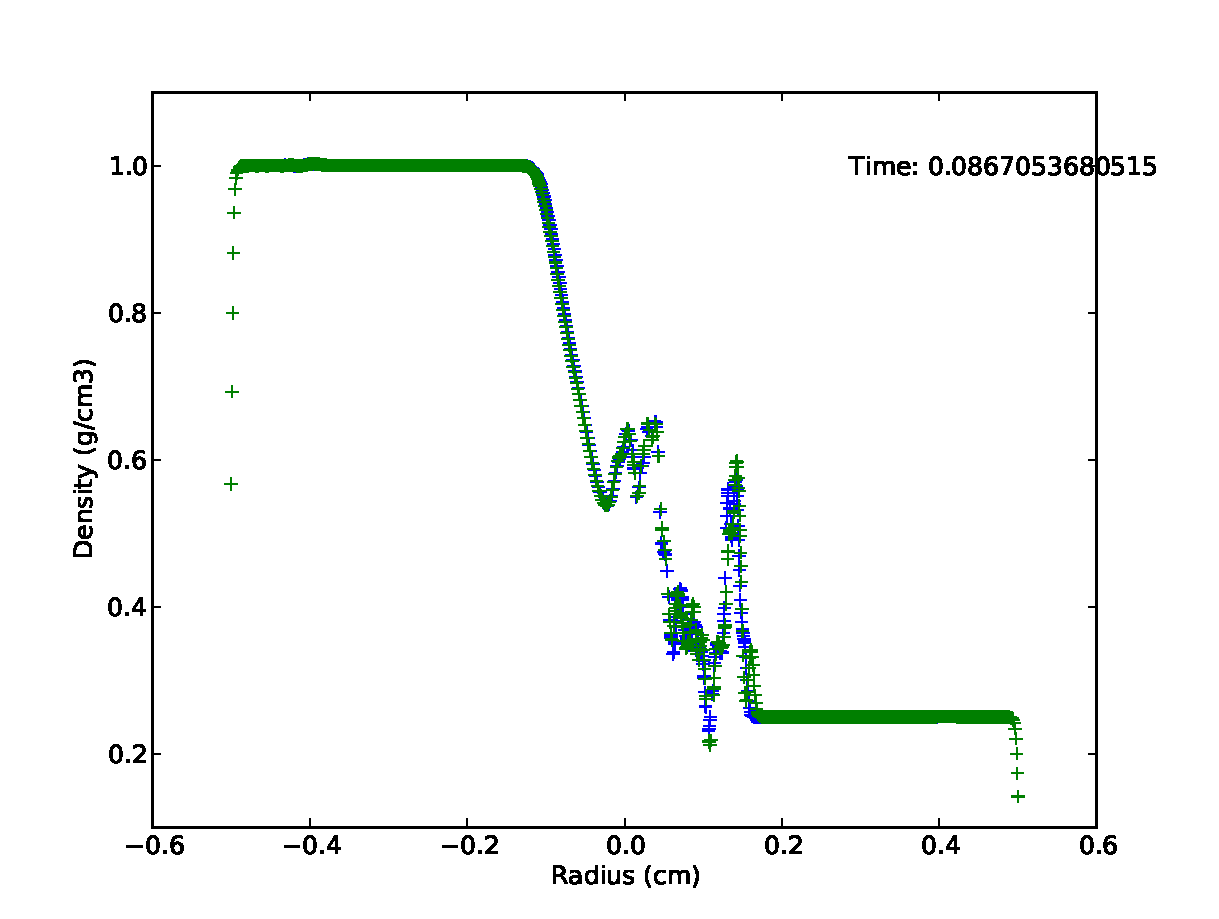
\includegraphics[width=0.5\textwidth]{Shock-100.pdf}
\label{fig:simpleplot}
\end{figure}

\end{document}
